\documentclass{beamer}
\usepackage[slovene]{babel}
\usepackage{textcomp}
\usepackage[utf8]{inputenc}
\usepackage{lmodern}
\usepackage[T1]{fontenc}
\usetheme{Warsaw}
\usepackage{graphicx}
\mode<presentation>
\usepackage{latexsym}
\usepackage{amsmath}
\usepackage{amssymb}
\newtheorem{izrek}{Izrek}


\title[dolga predstavitev diplomskega dela]{Posplošena diskriminantna analiza z uporabo posplošenega singularnega razcepa } 
\author[Jernej Banevec]{Jernej Banevec\\
\medskip
{\small Mentor: izred. prof. dr. Marjeta Knez1}
}
\institute[FMF] 
{
Fakulteta za matematiko in fiziko\\ 
\medskip
\textit{dolga predstavitev diplomskega dela} 
}
\date{3.4.2017} 

\begin{document}


\begin{frame}
\titlepage
\end{frame}

\begin{frame}
\frametitle{Pregled vsebine} 
\tableofcontents 
\end{frame}


\section{Posplošena diskriminantna analiza}

\begin{frame}
\frametitle{Posplošena diskriminantna analiza}
\begin{itemize}
\item Posplošitev linearne diskriminantne analize
\item Ena zelo uporabljenih statističnih metod
\item Oblike podatkov:
\begin{itemize}
\item Združeni v matriki $A \in \mathbb{R}^{mxn}$
\item m \ldots dimenzija posamezne meritve
\item n \ldots število meritev oz. podatkov
\item Podatki grupirani v k razredov oz. gruč
\end{itemize}
\end{itemize}
\end{frame}


\begin{frame}
\frametitle{Posplošena diskriminantna analiza}
\begin{itemize}
\item Iščemo preslikavo $$G : \mathbb{R}^m \rightarrow \mathbb{R}^\ell ,$$ kjer je $\ell \leqslant m - 1$
\item Cilj:
\begin{itemize}
\item Ohraniti razporejenost razredov
\item Zmanjšati razpršenost podatkov znotraj razredov
\item Povečati razlike med razredi
\end{itemize}
\end{itemize}
\end{frame}


\begin{frame}
\frametitle{Primerjava dobra proti slabi preslikavi}
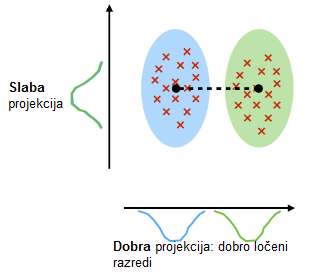
\includegraphics[scale = 0.85]{dobra-slaba}
\end{frame}


\begin{frame}
\frametitle{Definicije}
\begin{itemize}
\item Centroid i-tega razreda: $c^{(i)} = \frac{1}{n_i} \sum_{j \in N_i} a_j$
\item Centroid celotnih podatkov: $c = \frac{1}{n} \sum_{j = 1}^{n} a_j$
\item $H_W = [A_1 - c^{(1)}e^{(1)^T}, \ldots, A_k - c^{(k)}e^{(k)^T}]$
\item $H_B = [(c^{(1)} - c)e^{(1)^T}, \ldots,(c^{(k)} - c) e^{(k)^T}]$
\item $e^{(i)} = (1,\ldots, 1) ^T \in \mathbb{R}^{ n_i x 1 }$
\end{itemize}
\end{frame}


\begin{frame}
\frametitle{Definicije}
\begin{itemize}
\item Matrika razpršenosti podatkov znotraj razreda: $$S_W = \sum_{i = 1}^{k} \sum_{j \in N_i}(a_j - c^{(i)})(a_j - c^{(i)})^T = H_W H_W^T$$
\item Matrika razlik med razredi: $$S_B = \sum_{i = 1}^{k} n_i ( c^{(i)} - c)( c^{(i)} - c)^T = H_B H_B^T$$
\item Matrika celotne razpršenosti: $$S_M = S_W + S_B$$
\item Tu so vse matrike elementi $\mathbb{R}^{mxm}$
\end{itemize}
\end{frame}


\begin{frame}
\frametitle{Definicije}
\begin{itemize}
\item Preslikava $S_W$ na prostor dimenzije $\ell$ : $$ S_{W}^{\ell} = G^T S_W G$$
\item Preslikava $S_B$ na prostor dimenzije $\ell$ : $$ S_{B}^{\ell} = G^T S_B G$$
\item Preslikava $S_M$ na prostor dimenzije $\ell$ : $$ S_{M}^{\ell} = G^T S_M G$$
\item Tu so vse matrike elementi $\mathbb{R}^{ \ell x \ell } $
\item Preslikamo tudi matriko podatkov $A$: $G^T A$
\end{itemize}
\end{frame}



\section{Posplošena diskriminantna analiza kot optimizacijski problem}

\begin{frame}
\frametitle{Posplošena diskriminantna analiza kot optimizacijski problem}
\begin{itemize}
%\item $ sled(S_W) = \sum_{i = 1}^{k} \sum_{j \in N_i}(a_j - c^{(i)})^T(a_j - c^{(i)}) = \sum_{i = 1}^{k} \sum_{j \in N_i} || a_j - c^{(i)}||_2^2$
%\item $ sled(S_B) = \sum_{i = 1}^{k}n_i( c^{(i)} - c)^T( c^{(i)} - c) = \sum_{i = 1}^{k} n_i || c^{(i)} - c||_2^2$
\item $ sled(S_W) = \sum_{i = 1}^{k} \sum_{j \in N_i} || a_j - c^{(i)}||_2^2$
\item $ sled(S_B) = \sum_{i = 1}^{k} n_i || c^{(i)} - c||_2^2$
\item Želimo:
\begin{itemize}
\item povečati $sled(S_B^\ell)$
\item zmanjšati $sled(S_W^\ell)$
\end{itemize}
\item Dobimo optimizacijski problem, pri katerem iščemo takšno preslikavo $G$, ki maksimizira
$$sled( G^T S_B G) / sled( G^T S_W G) \approx sled((S_W^\ell)^{-1}S_B^\ell)$$
\item Kriterija ne moremo uporabiti ko $S_W$ singularna oz. neobrnljiva
\end{itemize}
\end{frame}


\section{Iskanje optimalnega G}
\begin{frame}
\frametitle{$S_W$ obrnljiva} 
\begin{itemize}
\item Definicija:
\begin{itemize}
\item $S_1 = S_B$
\item $S_2 = S_W$
\end{itemize}
\item Tudi simetrično pozitivno definitna \textrightarrow razcep Choleskega $S_2 = VV^T$
\item Posplošen problem lastnih vrednosti $S_1 x = \lambda S_2 x$
\item Označimo $J_1(G) = sled((G^T S_2 G)^{-1}G^T S_1 G)$
\item Iščemo $G  \in \mathbb{R}^{ m x \ell }$, kjer $J_1(G)$ maksimalen
\item $max_G J_1(G) \leq \lambda_1 + \lambda_2 + \ldots +  \lambda_q = sled(S_2^{-1} S_1)$
\item Optimalen $G = X \begin{bmatrix} 
I_\ell \\
0 
\end{bmatrix}$
\end{itemize}
\end{frame}

\section{Posplošeni singularni razcep}

\begin{frame}
\frametitle{Singularni razcep}
\begin{itemize}
\item Originalna definicija posplošenega singularnega razcepa (Van Loan)
\begin{izrek}[Singularni razcep]
\label{izrek:SVD} Za matriki $K_A \in \mathbb{R}^{pxm}$ z $p \geq m$ in $K_B \in \mathbb{R}^{nxm}$ obstajata ortogonalni matriki $U \in \mathbb{R}^{pxp}$ in $V \in \mathbb{R}^{nxn}$ ter nesingularna matrika $X \in \mathbb{R}^{mxm}$, da velja $$ U^T K_A X = diag(\alpha_1,..., \alpha_m) \ \text{in} \ V^T K_B X = diag(\beta_1,..., \beta_q) $$ kjer $q = min(n,m)$, $\alpha_i \geq 0$ za $1 \leq i \leq m$ in  $\beta_i \geq 0$ za  $1 \leq i \leq q$.
\end{izrek}
\end{itemize}
\end{frame}

\begin{frame}
\frametitle{Posplošeni singularni razcep}
\begin{izrek}[Posplošeni singularni razcep]
\label{izrek:GSVD} Naj bosta dani matriki $K_A \in \mathbb{R}^{pxm}$ in $K_B \in \mathbb{R}^{nxm}$. Potem za $K = \left(\begin{array}{c} K_A \\ K_B \end{array}\right)$ in $t = rang(K)$ obstajajo ortogonalne matrike $U \in \mathbb{R}^{pxp}$, $V \in \mathbb{R}^{nxn}$, $W \in \mathbb{R}^{txt}$ in $Q \in \mathbb{R}^{mxm}$, da velja: 
$$U^T K_A Q = \Sigma_A  \left(\begin{array}{cc} W^T R, & 0 \end{array}\right) \text{in}\hspace{2.5mm} V^T K_B Q = \Sigma_B  \left(\begin{array}{cc} W^T R, & 0 \end{array}\right),$$ kjer je 
$\Sigma_A = \begin{pmatrix} 
I_A &  & \\
 & D_A & \\
 & & 0_A  
\end{pmatrix}$ in
$\Sigma_B = \begin{pmatrix} 
0_B &  & \\
 & D_B & \\
 & & I_B  
\end{pmatrix}$ in
\end{izrek}
\end{frame}

\begin{frame}
\frametitle{Posplošeni singularni razcep nadaljevanje}
\begin{izrek}[Posplošeni singularni razcep]
\label{izrek:GSVD1} $R \in \mathbb{R}^{txt}$ nesingularna, matriki $I_A \in \mathbb{R}^{rxr}$ in $I_B \in \mathbb{R}^{(t-r-s)x(t-r-s)}$ identični matriki, kjer je 
$$r = rang(K) - rang(K_B)\hspace{2mm} \text{in}\hspace{2mm} s = rang(K_A) + rang(K_B) - rang(K),$$
$0_A \in \mathbb{R}^{(p-r-s)x(t-r-s)}$ in $0_B \in \mathbb{R}^{(n-t+r)xr}$,
$D_A = diag(\alpha_{r+1},..., \alpha_{r+s})$ in $D_B = diag(\beta_{r+1},..., \beta_{r+s})$, ki zadoščajo pogoju:
$$1 > \alpha_{r+1} \geq \ldots \geq \alpha_{r+s} > 0  \hspace{4mm} \text{in} \hspace{4mm} 1 < \beta_{r+1} \leq \ldots \leq \beta_{r+s} < 0$$
pri $\alpha_i^2 + \beta_i^2 = 1$ za $ i = r+1,\ldots, r+s$
\vspace{-2mm} 
\end{izrek}
\end{frame}

\begin{frame}
\frametitle{Posplošeni singularni razcep za nadaljno uporabo}
Zgornja izreka povežemo s posplošitvijo singularnega razcepa Van Loana v obliko $$U^T K_A X = \left(\begin{array}{cc} \Sigma_A, & 0 \end{array}\right) \text{in} V^T K_B X = \left(\begin{array}{cc} \Sigma_B, & 0 \end{array}\right), $$ kjer je $$X = Q  \left(\begin{array}{cc} R^{-1}W & 0\\ 0 & I \end{array}\right) .$$
\end{frame}

\section{Iskanje optimalnega G z uporabo GSVD}
\begin{frame}
\frametitle{$S_W$ poljubna} 
\begin{itemize}
\item $G$ poiščemo z uporabo GSVD na $K = \left(\begin{array}{c} H_B^T \\ H_W^T \end{array}\right) \in \mathbb{R}^{2nxm}$
\item Dobimo 
\begin{itemize}
\item $H_B^T = U \left(\begin{array}{cc} \Sigma_A, & 0 \end{array}\right) X^{-1} $
\item $H_W^T = V \left(\begin{array}{cc} \Sigma_B, & 0 \end{array}\right) X^{-1} $
\end{itemize}
\item Dodatno definirajmo:
\begin{itemize}
\item $\alpha_i = 1, \beta_i = 0$ za $i = 1,2, \ldots, r$ 
\item $\alpha_i = 0, \beta_i = 1$ za $i = r+s+1, \ldots, t$ 
\end{itemize}
\item Dobimo: $\beta_i ^2  H_W H_W^T x_i = \alpha_i^2  H_B H_B^T x_i$
\end{itemize}
\end{frame}

\begin{frame}
\frametitle{$S_W$ poljubna} 
\begin{itemize}
\item $H_W^T$ polnega ranga:
\begin{itemize}
\item Rang torej $m$
\item $S_W$ torej obrnljiva
\item $r = 0$ in $t = m$ 
\item $\beta_1, \ldots, \beta_m > 0$
\item Posplošeni problem lastnih vrednosti $H_W H_W^T x_i = \frac{\alpha_i^2}{\beta_i ^2} H_B H_B^T x_i$
\end{itemize}
\item $H_W^T$ ni polnega ranga:
\begin{itemize}
\item $G$ tudi tu iz prvih $\ell$ stolpcev matrike $X$
\end{itemize}
\end{itemize}
\end{frame}


\section{Algoritem LDA/GSVD}
\begin{frame}
\frametitle{Algoritem LDA/GSVD} 
Algoritem, ki za matriko podatkov $A \in \mathbb{R}^{ m x n } $ s $k$ razredi ustvari matriko $G  \in \mathbb{R}^{ m x \ell }$, ki ohranja oblike razredov v manj-dimenzionalnem prostoru in kjer $\ell < k$, z uporabo optimizacije
$$J_1(G) = sled((G^T S_W G)^{-1}G^T S_B G)$$

\end{frame}

\begin{frame}
\frametitle{Algoritem LDA/GSVD} 
\begin{enumerate}
\item Iz $A$ izračunamo $H_B$ in $H_W$
\item Za $K = \left(\begin{array}{c} H_B^T \\ H_W^T \end{array}\right) \in \mathbb{R}^{2nxm}$ izračunamo singularni razcep:$$ P^T K Q =\left(\begin{array}{cc} R & 0\\ 0 & 0 \end{array}\right)$$
\item $t = rang(K)$
\item Izračunamo $W$ iz singularnega razcepa za $P(1:n, 1:t)$:$$U^T P(1:n, 1:t) W = \Sigma_A$$
\item $G$ sestavimo iz prvih $\ell$ stolpcev matrike $X = \left(\begin{array}{cc} R^{-1}W & 0\\ 0 & I \end{array}\right)$
\end{enumerate}
\end{frame}


\section{Zgled}

\begin{frame}
\frametitle{Zgled - roža Iris}
\begin{itemize}
\item Precej poznan zgled
\item Trije razredi:
\begin{enumerate}
\item Iris - setosa
\item Iris - versicolor
\item Iris - virginica
\end{enumerate}
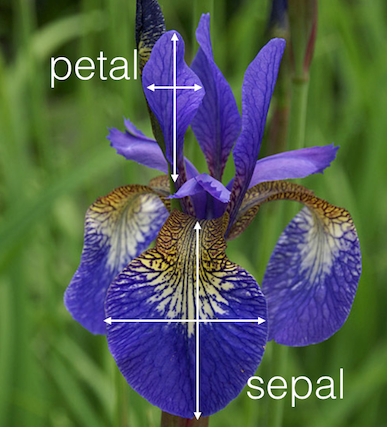
\includegraphics[scale = 0.30]{Iris1}
\end{itemize}
\end{frame}


\begin{frame}
\frametitle{Zgled - roža Iris}
\begin{itemize}
\item Podatki:
\[
A =
\begin{bmatrix}
	a_{1_{\text{sepal  length}}} & a_{2_{\text{sepal  length}}} & \cdots  & a_{150_{\text{sepal  length}}} \\
	a_{1_{\text{sepal  width}}} & a_{2_{\text{sepal width}}} & \cdots  & a_{150_{\text{sepal  width}}} \\
	a_{1_{\text{petal  length}}} & a_{2_{\text{petal  length}}} & \cdots  & a_{150_{\text{petal  length}}} \\
	a_{1_{\text{petal  width}}} & a_{2_{\text{petal  width}}} & \cdots  & a_{150_{\text{petal  width}}}
\end{bmatrix}
\]
\end{itemize}
\end{frame}

\begin{frame}
\frametitle{Zgled - roža Iris}
\begin{itemize}
\item Na teh podatkih uporabimo posplošeno diskriminantno analizo
\begin{enumerate}
\item Računanje centroidov
\item Računanje matrik razpršenosti podatkov
\item Lastni razcep $(S_W)^{-1}S_B$
\item Urejanje lastnih vrednosti (po parih z vektorji)
\item Transformiranje na nov podprostor
\end{enumerate}
\end{itemize}
\end{frame}

\begin{frame}
\frametitle{Zgled - roža Iris}
\begin{itemize}
\item Slikamo na 2-dimenzionalen (pod)prostor
\item Dobimo sledečo sliko:
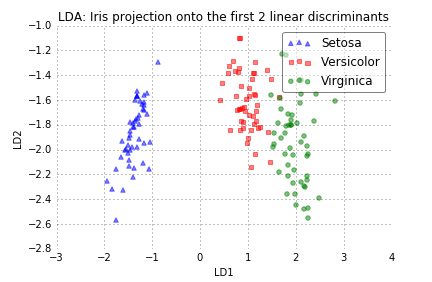
\includegraphics[scale = 0.65]{Iris3}
\end{itemize}
\end{frame}


\section{Viri}

\begin{frame}
\frametitle{Viri}
\begin{itemize}
\item Howland P. in Park H., Generalizing discriminant analysis using the generalizen singular value decomposition. TPAMI. 2004, 26, 8, 995-1006
\item Jieping Ye, Characterization of a Family of Algorithms for Generalized Discriminant Analysis on Undersampled Problems. Journal of Machine Learning Research. 2005, 6, 483–502
\end{itemize}
\end{frame}

\end{document}
